\documentclass[border=5pt, multi, tikz]{standalone}
\usetikzlibrary{quotes,arrows.meta}

\usepackage{xcolor}
\definecolor{morange}{RGB}{255,127,14}
\definecolor{mblue}{RGB}{31,119,180}
\definecolor{mred}{RGB}{214,39,40}
\definecolor{mpurple}{RGB}{148,103,189}
\definecolor{mgreen}{RGB}{44,160,44}

\begin{document}
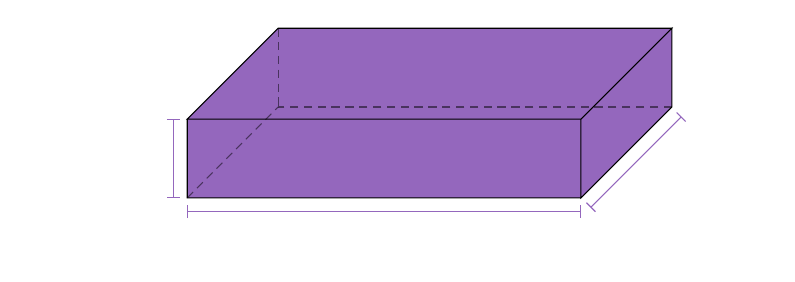
\begin{tikzpicture}[every edge quotes/.append style={auto, text=white}]
  \pgfmathsetmacro{\cubex}{5}
  \pgfmathsetmacro{\cubey}{1}
  \pgfmathsetmacro{\cubez}{3}
  \draw [draw=black, every edge/.append style={draw=black, densely dashed, opacity=.5}, fill=mpurple]
    (0,0,0) coordinate (o) -- ++(-\cubex,0,0) coordinate (a) -- ++(0,-\cubey,0) coordinate (b) edge coordinate [pos=1] (g) ++(0,0,-\cubez)  -- ++(\cubex,0,0) coordinate (c) -- cycle
    (o) -- ++(0,0,-\cubez) coordinate (d) -- ++(0,-\cubey,0) coordinate (e) edge (g) -- (c) -- cycle
    (o) -- (a) -- ++(0,0,-\cubez) coordinate (f) edge (g) -- (d) -- cycle;
  \path [every edge/.append style={draw=mpurple, |-|}]
    (b) +(0,-5pt) coordinate (b1) edge ["\texttt{input\_time\_steps}"'] (b1 -| c)
    (b) +(-5pt,0) coordinate (b2) edge ["\texttt{input\_dim}"] (b2 |- a)
    (c) +(3.5pt,-3.5pt) coordinate (c2) edge ["\texttt{n\_params}"'] ([xshift=3.5pt,yshift=-3.5pt]e)
    ;
\end{tikzpicture}
\end{document}